\section{数字集成电路设计中的问题}
在1960年左右,Gordon Moore(摩尔,当时在Fairchild即仙童公司工作,而后成为Intel公司的合伙奠基人)预见:能够在一个单片上集成的晶体管数目将随时间按指数规律增长。这一预见,后来被成为\uwave{摩尔定律}(Moore Law)。具体而言,处理器和存储器的集成密度每1-2年就会翻一倍,集成电路在过去几十年间都遵循着摩尔定律快速发展,直至近几年才逐渐放缓。

毫无疑问的是,摩尔定律对如何设计数字电路产生了巨大影响。早期的数字电路设计完全是手工操作,每个晶体管都要画出其版图并且一个一个地优化并仔细放入它周围的四邻之间,例如\xref{subsec:晶体管}提到的第一代微处理器Intel 4004就是这一手工设计出来的,共有2300个晶体管。\xref{fig:Intel 4004微处理器}充分展示了这一点,它显示了Intel 4004的设计。然而,摩尔定律趋势下,集成密度越来越高,晶体管数量越来越多,手工设计,无论从设计时间还是设计成本上都不再可行。

因此,设计者已经越来越遵循比较适合设计自动化的严格设计方法和策略。现今一个电路的设计是按层次化方法进行的,处理是许多模块的集合,模块又有更多的子模块构成,模块尽可能重复使用以减少设计压力并提高设计一次成功的机会。这一层次化的步骤完全可行的事实是数字电路设计成功的关键,也是当今,我们能够设计出如此复杂的数字电路的根本原因。

层次化的设计观点的关键在于“抽象”,即在每个设计层次上,一个复杂模块的内部细节可以用一个黑盒模型代替,模型包含了在该层次上处理这一模块所需要的所有信息。例如当设计者实现了一个非门,它就可以精确的放入这样一个模型:输入$1$则输出$0$,输入$0$则输出$1$。通常来说,非门的性能只是略受它在一个较大系统中运用方式的影响,因此在任何情况下,非门都可以被考虑成一个具有已知特性的黑盒。由于系统设计者并不必了解这个黑盒子内部的细节,例如非门是如何由MOS管构成等等,从而大大减少了设计的复杂性。这种设计方式是很有效的,每一层次的设计者,只需要面对自己所在层次的若干用少量参数表征内部特性的部件模型,只需要处理这些部件模型之间的连接和关系,而不必关心数不清的底层单元。

\begin{Figure}[Intel 4004微处理器]
    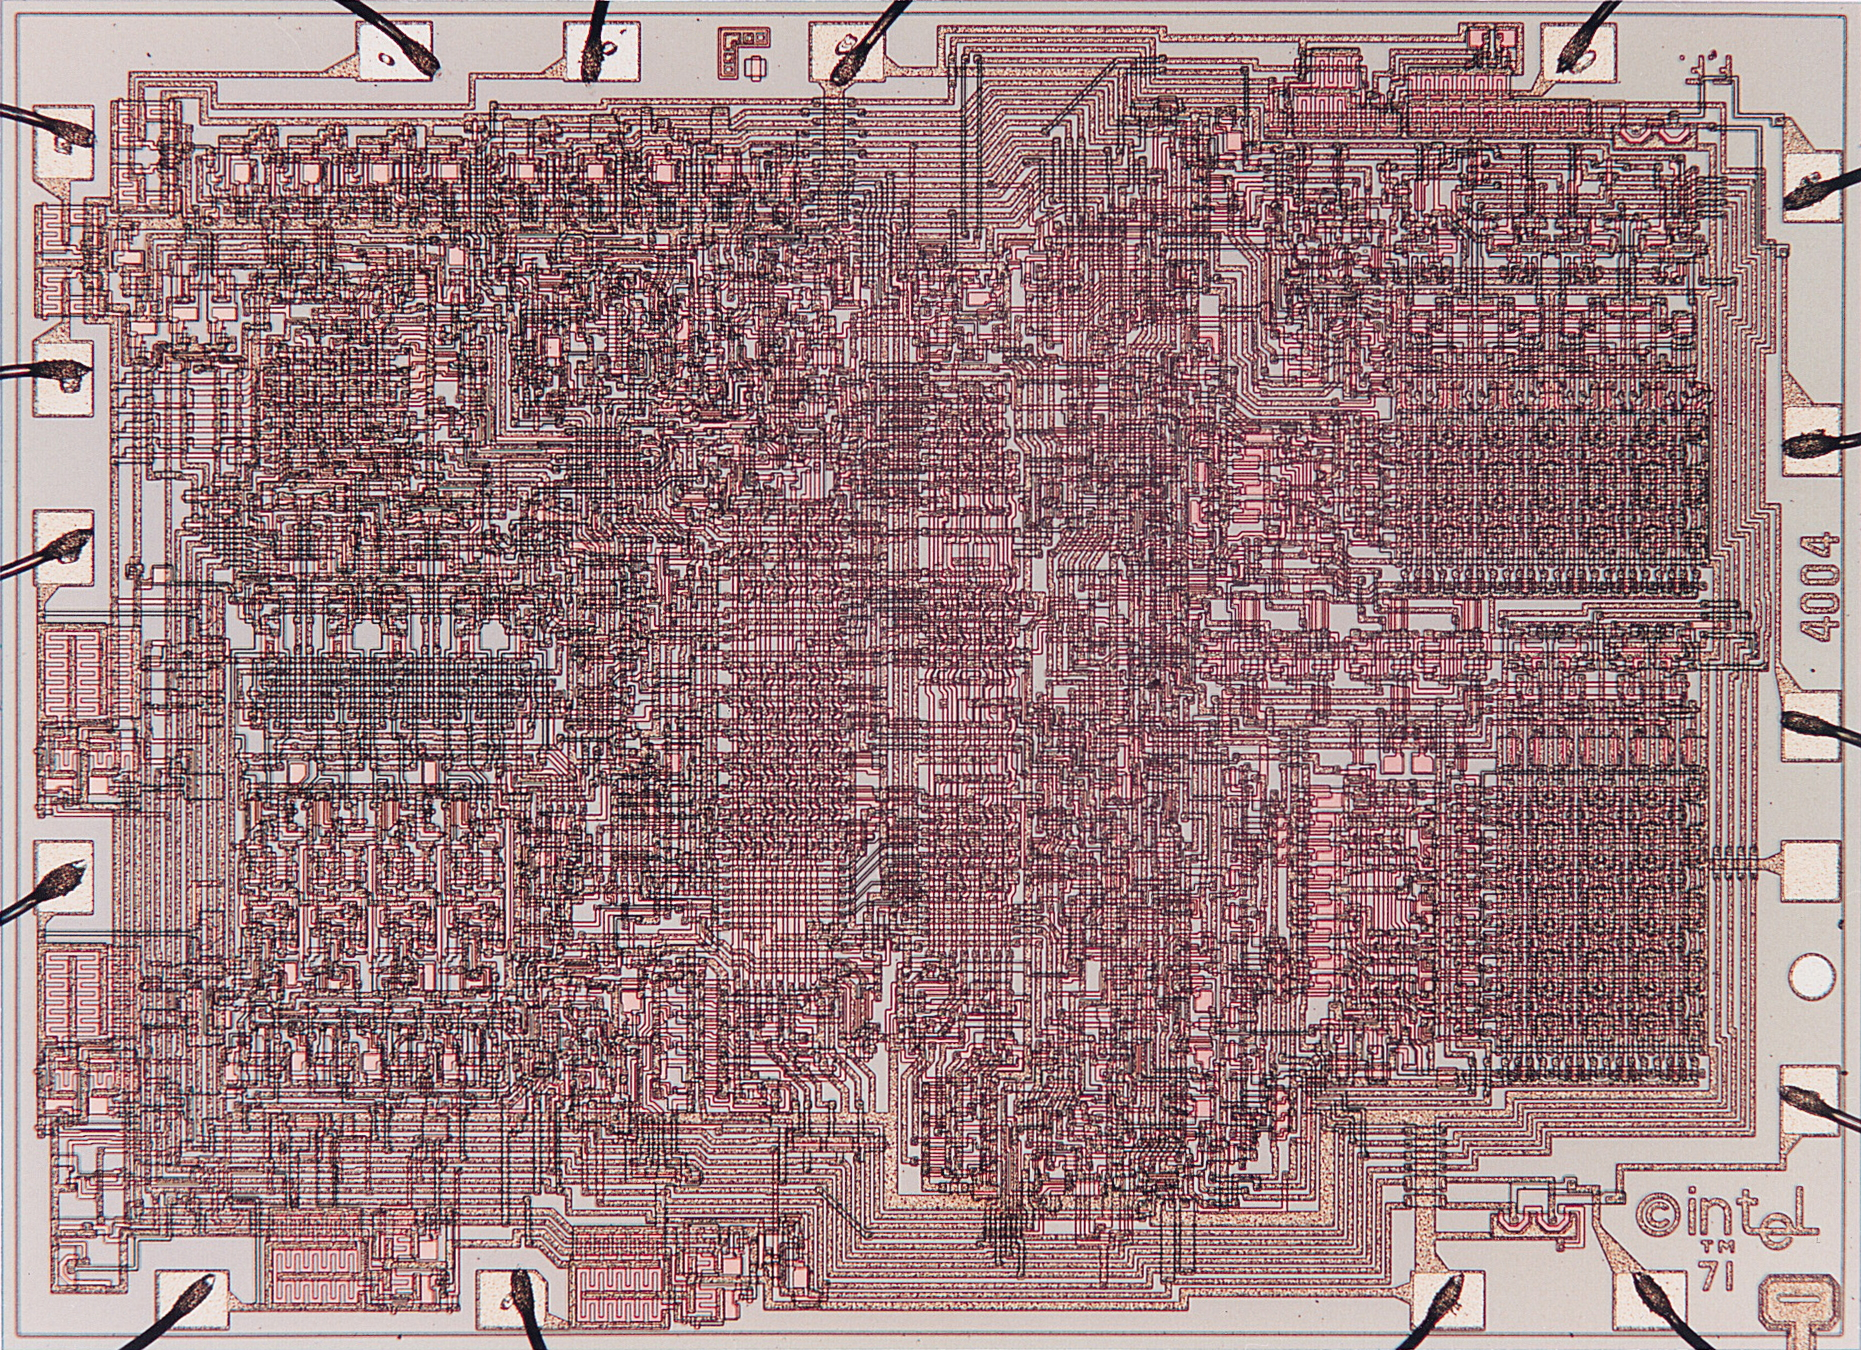
\includegraphics[width=1\linewidth]{image/4004_die_large.jpg}
\end{Figure}

这里应当指出的是,层次化的设计观点只在数字设计中可行,而在模拟设计中不可行。这很大程度上就是因为,模拟设计中无法抽象出简单的模型,模块的性能会很大程度上受到它的使用方式的影响,这也是为何人们并不那么乐意设计规模非常大的的模拟集成电路的原因。

这里在\xref{fig:数字电路设计的抽象层次}中绘制了数字电路设计的典型抽象层次
\begin{enumerate}
    \item 器件
    \item 电路
    \item 门
    \item 模块
    \item 系统
\end{enumerate}
半导体器件是一个具有复杂特性的实体,从来没有哪个电路设计者在设计一个数字门时会认真考虑决定器件特性的固体物理方程,相反,它会利用一个简化模型来恰当描述这个器件的输入输出特性。例如,非门可以用这个门的逻辑表达式$Z=\bar{A}$、它的版图边框、输入和输出的终端位置、输入和输出间的延时等参数来恰当描述。这就是层次化设计思想的具体表现。

\begin{Figure}[数字电路设计的抽象层次]
    \includegraphics[width=1\linewidth]{build/Chapter01B_01.fig.pdf}
\end{Figure}

层次化设计类似于运用软件子程序库的软件设计者。写一个大程序的人并不需要去了解这些子程序的内部细节,他唯一关心的,是调用其中一个模块并得到所希望的结果。想象一下,如果一个人必须从磁盘中一个一个地读取每个二进制位并保持它的正确性,而不是依赖于方便的“打开文件”和“取字符串”这样的操作函数,那么写一个软件程序将变得多么困难。

层次化的设计思想使精心构思的数字集成电路CAD平台的出现成为可能,没有CAD的帮助是不可能实现当前的设计复杂程度的。为了避免重复设计和重复验证一些常用的单元,如基本的逻辑门和运算模块及存储模块,设计者常会使用单元库,其中不仅包含单元的版图,还提供描述这些单元行为的数据。当所使用的模块存在于单元库时,模块的版图就可以自动生成。

前面的分析已经表明,层次化的设计方法已经有效解决了现代数字设计中存在的一些复杂性问题,那么。为什么我们还要关心数字电路设计呢?实际上,现实是比较复杂的,存在以下各种理由可以说明为什么数字电路的深刻理解仍将是极为重要的
\begin{enumerate}
    \item 第一,仍然必须有人来设计和实现单元库。半导体工艺年复一年的持续发展,工艺的变化平均每两年就会发生一次,工艺每一次变化都要求重新设计单元库。
    \item 第二,单元的模型建立需要对它的内部操作有深刻的理解。
    \item 第三,单元库在追求极致性能时,就不再那么吸引人了。类似于编写软件程序,当执行效率是关键因素是,编程着倾向于编写“定制”程序而不是使用“通用”的函数。
    \item 第四,以抽象为基础的层次化设计方法实际上只在一定程度上是正确的。随着工艺的提升,数字电路中也会遇到类似模拟电路的问题。模块的性能可以明显受它与其他环境连接方式的影响。模块间的互连线也会产生延时,因为它们会引起寄生电容和寄生电阻。
\end{enumerate}

因此,数字集成电路这门课程的目标是,在数字设计的抽象思想和作为其基础的数字电路间建立一座桥梁。在掌握数字设计方法的同时,也能对数字电路的底层原理有较深入的了解。